% Generated by scripts.reports.metric_conditioned_paper_slice; do not edit.
\subsection{Completed loss-conditioned comparison}
The three objectives selected 2 distinct frozen institutional designs under otherwise identical search conditions. The identity of the best frozen system changed across held-out scoring losses, a descriptive rank reversal between the frozen designs. All 9 paired held-out loss contrasts have 95\% intervals containing zero, so five seeds do not establish stable pairwise superiority. The topic-entropy and review-burden objectives selected the same design; their arm-labelled held-out trajectories are independent stochastic repetitions, not distinct institutional systems.
The experimental intervention is the optimization \code{LossSpec}; the simulator, design space, optimizer, budget, and seeds are held fixed. The proxy objectives are contrasts, not normative recommendations, and the report-only protocol selects no universal winner.
\begin{table}[t]
\caption{Frozen systems and own-objective generalization. Intervals are exact nonparametric 95\% bootstrap percentile intervals for the complete LossSpec aggregate over the 5 common held-out seeds.}
\label{tab:metric-conditioned-heldout-winners}
\centering\small
\begin{tabular}{lrrrr}
\toprule
Objective & Proposal & Development & Held-out [95\% CI] & Gap \\
\midrule
Participation-review & 2 & 0.322 & 0.295 [0.229, 0.350] & -0.026 \\
Topic-entropy proxy & 1 & -1.697 & -1.712 [-1.854, -1.563] & -0.015 \\
Review-burden proxy & 1 & 1.669 & 1.454 [1.335, 1.585] & -0.215 \\
\bottomrule
\end{tabular}
\end{table}
\begin{table}[t]
\caption{Institutional parameters of the three frozen systems. Differences are consequences of changing the optimization objective under a shared search protocol.}
\label{tab:metric-conditioned-designs}
\centering\small
\resizebox{\linewidth}{!}{%
\begin{tabular}{llll}
\toprule
Parameter & Participation-review & Topic-entropy proxy & Review-burden proxy \\
\midrule
acceptance\_rate & 0.496777 & 0.113159 & 0.113159 \\
funding\_application\_cost & 1 & 1 & 1 \\
funding\_budget\_slots\_frac & 0.390677 & 0.327413 & 0.327413 \\
resubmission\_cost & 12.8905 & 16.3863 & 16.3863 \\
review\_policy & persona & standardized & standardized \\
reviewer\_capacity & 8 & 2 & 2 \\
reviewer\_matching & topic & random & random \\
reviews\_per\_paper & 3 & 4 & 4 \\
\bottomrule
\end{tabular}%
}
\end{table}
\begin{figure}[t]
\centering
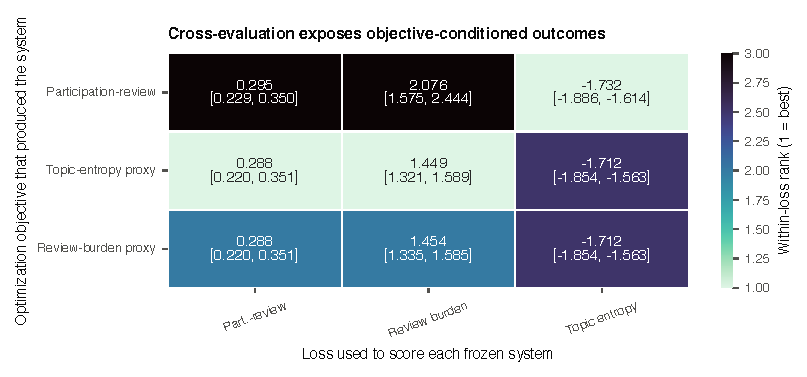
\includegraphics[width=0.92\linewidth]{generated/metric-conditioned/figures/metric-conditioned-cross-evaluation.pdf}
\caption{Cross-evaluation of frozen systems. Annotations give the held-out LossSpec aggregate and its exact-bootstrap 95\% interval; color gives within-loss rank because loss units differ.}
\label{fig:metric-conditioned-cross-evaluation}
\end{figure}
\begin{figure}[t]
\centering
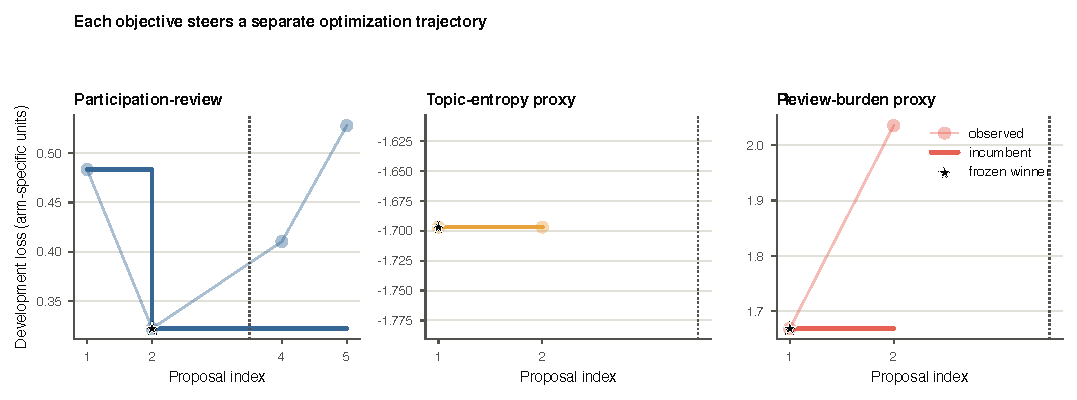
\includegraphics[width=\linewidth]{generated/metric-conditioned/figures/metric-conditioned-objective-trajectories.pdf}
\caption{Development trajectories in arm-specific units. Stars mark the simultaneously frozen winners.}
\label{fig:metric-conditioned-trajectories}
\end{figure}
\begin{figure}[t]
\centering
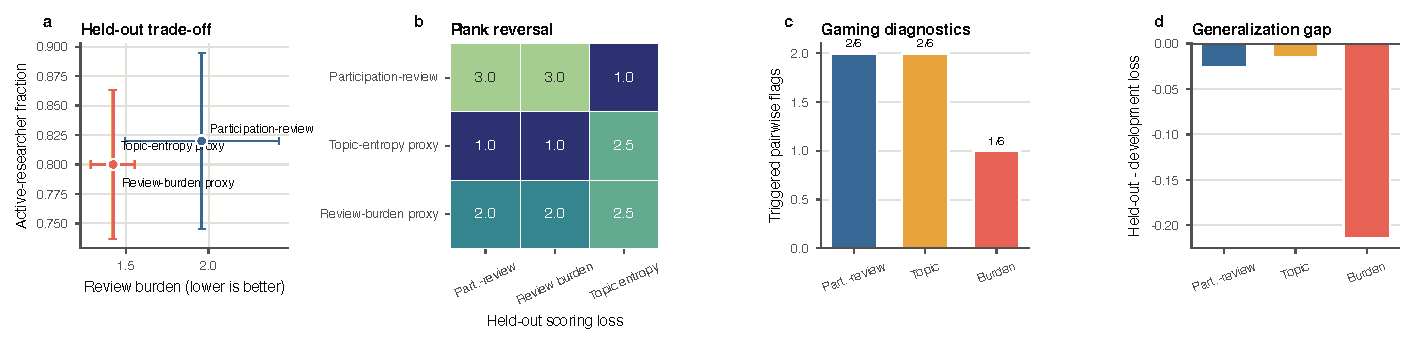
\includegraphics[width=\linewidth]{generated/metric-conditioned/figures/metric-conditioned-tradeoff-rank-generalization.pdf}
\caption{Held-out trade-off, rank reversal, proxy-gaming flags, and generalization diagnostics. Flags are diagnostics rather than validity failures or promotion vetoes; the panels characterize objective dependence rather than a universal optimum.}
\label{fig:metric-conditioned-diagnostics}
\end{figure}
\paragraph{Runtime and provenance.}
The slice contains 45 logical optimization runs, 29 physical optimization runs, 16 adopted logical runs, 15 terminal technical failures retained without numeric penalties, and 15 held-out runs (at least 52.35 recorded attempt-runtime hours; 1 interrupted attempt(s) lack wall time). Source commit: \code{1078279d1ce833afe9ffb6b7c262da15357b76ab}; winner freeze: \code{254c3366e921787ad6a36776801b1cb3b278e2cb36ef247da4cb127b6459244d}.
